\documentclass[a4paper,12pt]{article}
\usepackage[pdftex]{graphicx}

\pagestyle{empty} \setlength{\parindent}{0mm}
\addtolength{\topmargin}{-0.5in} \setlength{\textheight}{9in}
\addtolength{\textwidth}{1in} \addtolength{\oddsidemargin}{-0.5in}

\begin{document}

{\bf Name:} Matt Forbes \\
{\bf Partner:} Stuart  \\ 
{\bf Section:} Phys 233 - Thursday \\
{\bf TA:} Ellis Roe  \\ \\ 
{\bf Lab 3:} Standing Waves \\

\section{Purpose}
This week's lab was an introduction to wave interference and standing
waves. Again, the format was three separate experiments (exercises)
split in to three lab stations. First, we looked at a system with two
harmonic oscillators (carts connected by springs) and noticed two
types of resonance modes. Second, we observed resonance in a vibrating
string at each of its harmonic frequencies. Finally, we empirically
determined the relationship of each component that describes the
fundamental frequency of a vibrating string under tension.

\section{Procedure}
\subsection{Exercise 1}
Our station was setup with a low friction track with two carts
attached together by springs driven by an oscillating hanging
mass. Using a function generator, we were able to control the
frequency of the hanging mass which in turn changed the frequency of
the two carts. Our task was to estimate the two fundamental
frequencies of the system, each describing a mode of motion.

\subsection{Exercise 2}
Here we had a piece of string under tension which could be vibrated
via a driver at frequencies controlled by a function generator. Under
these conditions, and knowing the fact that $f_n = nf_1$, we
experimentally discovered the first six resonant frequencies,
comparing them to the theoretical values aforementioned.

\subsection{Exercise 3}
At this station, our setup was very similar to exercise two, although
we had much more control of the variables of the string. Using a
notched lever we were able to adjust the tension force, $T$, on the
string, by swapping out thicker/thinner wires, we could adjust the
density, $\mu$, and by moving the bridges we adjusted the length,
$l$. Within this exercise were three tasks, one for each parameter. In
each case, we held all parameters constant except one, and determined
the fundamental frequency in each one. In this we were could describe
the relationship between said variable and fundamental frequency.

\section{Data}
\subsection{Exercise 1}
The first mode , $f_1$, was found to have a period of about 2.3 $\pm$
0.05 seconds which is equal to 0.43 Hz. To minimize error, we changed
the amplitude of the oscillation by adjusting the moment arm on the
oscillating hanging mass. \\

For $f_2$, the second mode, we found the period to be 1.36 $\pm$ 0.05
seconds, equal to a frequency of 0.74 Hz. \\

Finally, for the situation where only one cart is allowed to move, we
measured a period of 1.75 $\pm$ 0.05 seconds, giving $f_0$ = 0.57
Hz. 

\subsection{Exercise 2}
Here are the frequencies of the fundamental frequency and following 5
harmonics for the string. Note the following values have an error of
about $\pm$ 0.5 Hz. \\

$f_1$ = 24 Hz \\
$f_2$ = 47.9 Hz \\
$f_3$ = 72.9 Hz \\
$f_4$ = 95.5 Hz \\
$f_5$ = 118.5 Hz \\
$f_6$ = 142.5 Hz \\

\newpage

The following graphs describe the shape of each harmonic frequency in
the same order as listed above (notice the decrease in amplitude.)
\begin{center}
    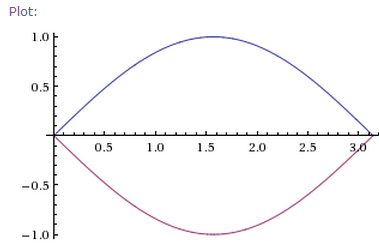
\includegraphics[width=2.5in, height=2in]{f1.PNG} \\
    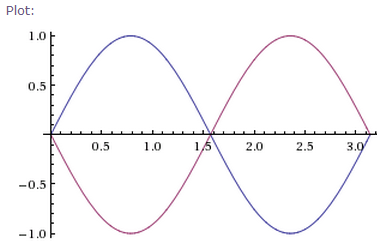
\includegraphics[width=2.5in, height=1.75in]{f2.PNG} \\
    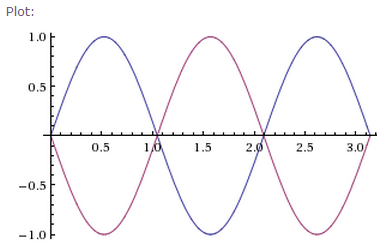
\includegraphics[width=2.5in, height=1.5in]{f3.PNG} \\
    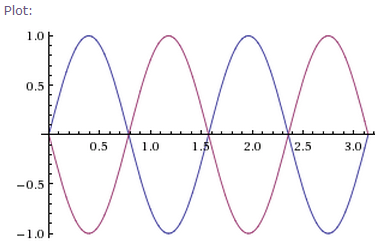
\includegraphics[width=2.5in, height=1.25in]{f4.PNG} \\
    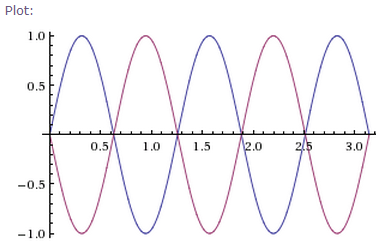
\includegraphics[width=2.5in, height=1in]{f5.PNG} \\
    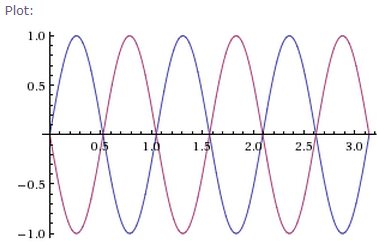
\includegraphics[width=2.5in, height=0.75in]{f6.PNG} \\
\end{center}

\subsection{Exercise 3}
The next three tables hold the data from the three sub-exercises of
exercise 3. Note that $l$ is length of the string, $T$ is the tension,
$\mu$ is the mass density of the string, and $f$ is the measured value
of the fundamental frequency for that particular setup. Also note that
our frequencies have an error of about $\pm$ 0.5 Hz \\

\begin{tabular}{c | c | c | c}
  $l$ & $T$ & $\mu$ & $f$ \\
  \hline
  60cm & 4Mg & $\mu_0$ & 237.6 Hz \\
  50cm & 4Mg & $\mu_0$ & 278.2 Hz \\
  40cm & 4Mg & $\mu_0$ & 347.4 Hz \\
  30cm & 4Mg & $\mu_0$ & 453.8 Hz \\
\end{tabular}

\vspace{1cm}

\begin{tabular}{c | c | c | c}
  $l$ & $T$ & $\mu$ & $f$ \\
  \hline
  60cm & 4Mg & $\mu_0$ & 237.6 Hz \\
  60cm & 3Mg & $\mu_0$ & 196.0 Hz \\
  60cm & 2Mg & $\mu_0$ & 160.6 Hz \\
  60cm & 1Mg & $\mu_0$ & 112.6 Hz \\
\end{tabular}\\

\vspace{1cm}

\begin{tabular}{c | c | c | c}
  $l$ & $T$ & $\mu$ & $f$ \\
  \hline
  60cm & 4Mg & $\mu_0$ & 237.6 Hz \\
  60cm & 4Mg & $1.5 * 10^{-2}$ & 201.8 Hz \\
  60cm & 4Mg & $1.84 * 10^{-2}$ & 185.6 Hz \\
\end{tabular}

\section{Analysis}
\subsection{Exercise 1}
After measuring the fundamental frequency of each of the three modes
in this system: carts moving together ($f_1$), carts moving opposite
($f_2$), and only one cart moving ($f_0$), we were asked to compare these
to the theoretically predicted values using the expressions: \\

$f_0 = \frac{1}{2\pi}\sqrt{ \frac{2K}{m} }$
$f_1 = \frac{1}{2\pi}\sqrt{ \frac{K}{m} }$
$f_2 = \frac{1}{2\pi}\sqrt{ \frac{3K}{m} }$ \\

Using our experimental value for $f_0$, which was 0.57 Hz, we can solve
for $K/M = 6.45$. Using this in the other expressions yields: \\

$f_1$ = 0.4 Hz \\ 
$f_2$ = 0.7 Hz. \\

Both of these values lie within 0.05 Hz of our experimentally found
versions. Timing the period of an oscillation is tricky to do by eye
with a stop watch, which most likely accounted for the majority of the
error in our approximations. Also, it's possible friction played a
role as well.

\newpage

\subsection{Exercise 2}
In this exercise, we simply measured the fundamental frequency of the
oscillating string as well as the next five harmonics. Assuming our
measurement of the fundamental frequency was mostly accurate, the
expression $f_n = nf_1$ should provide values roughly equal to our
measurements for the following harmonics:

\vspace{0.5cm}

\begin{tabular}{c | c | c}
  $f_n$ & experimental & theoretical ($nf_1$) \\
  \hline
  $f_1$ & 24 Hz & 24 Hz\\
  $f_2$ & 47.9 Hz & 48 Hz \\
  $f_3$ & 72.9 Hz & 72 Hz \\
  $f_4$ & 95.5 Hz & 96 Hz \\
  $f_5$ & 118.5 Hz & 120 Hz \\
  $f_6$ & 142.5 Hz & 142 Hz \\
\end{tabular} 

\vspace{0.5cm}

As we can see above, our experimental values of the harmonics match up
quite well with the theoretically expected ones (within 1 Hz in the
worst case).

\subsection{Exercise 3}
Using the expression $\frac{1}{2l}\sqrt{\frac{T}{\mu}}$ we found the
theoretical values for each set of parameters in this exercise. Rather
than list out all of the parameters here, the table will simply
consist of our measured frequency and theoretical value associated
with it.

\vspace{0.5cm}

\begin{tabular}{c | c}
  $f$ experimental & $f$ theoretical \\
  \hline
  237.6 Hz & 220.592 Hz\\
  278.2 Hz & 264.71 Hz\\
  347.4 Hz & 330.888 Hz\\
  453.8 Hz & 441.183 Hz\\
  \hline 
  196.0 Hz & 191.038 Hz\\
  160.6 Hz & 155.982 Hz\\
  112.6 Hz & 110.296 Hz\\
  \hline
  201.8 Hz & 190.613 Hz\\
  185.6 Hz & 172.103 Hz\\
\end{tabular}

\vspace{0.5cm}

So, while our experimental values don't match up perfectly, there was
a lot of room for error in this experiment. With so many variables,
the actual values are not likely to match up perfectly. More
importantly, though, the trends are the same. In this first case, the
fundamental frequency was inversely proportional to the length
$l$. Secondly, it was directly proportional to the square root of the
tension force. Finally, it was inversely proportional to the square
root of the mass density. 

\section{Conclusion}
By completing the exercises of this lab in order, we were first
introduced to the fundamental frequency by observing different modes
of an oscillating system. Next we measured this fundamental frequency
and its harmonics in a vibrating string. Finally, in exercise three,
we are able to make very general observations about the relationships
between the fundamental frequencies and parameters of an oscillating
system (these were noted at the end of the analysis section.) 

\end{document}
